\section{Metamodel}
\label{sec:slco:metamodel}

An \SLCO model consists of a number of classes, objects, and channels, as shown by the partial metamodel in Figure~\ref{fig:slco:MMMain}.
Objects are instances of classes.
A class describes the structure and behavior of its instances.
It has ports and variables that define the structure of its instances and state machines that describe their behavior.
It is possible to specify the initial values of variables.
If no initial value is specified, integer variables are initialized to $0$, Boolean variables are initialized to \SLCOTrue, and string variables are initialized to the empty string.
The variables of a class are global variables in the sense that they can be used by all state machines that are part of the class.
Ports are used to connect channels to objects, and each port is connected to at most one channel.
The state machines that are part of a class can only send and receive signals via the ports of this class.
In case a class specifies that its instances consist of multiple state machines, these state machines operate in parallel.

\begin{figure}[hbt]
 \centering
 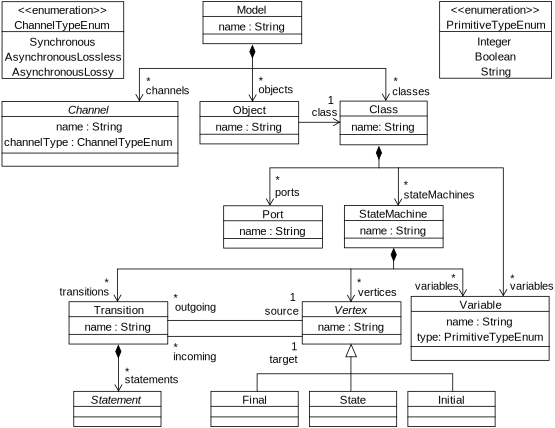
\includegraphics[scale=0.6]{slco/figs/metamodel/mm_slco_main}
 \caption{Main constructs of \SLCO}
 \label{fig:slco:MMMain}
\end{figure}

A state machine consists of variables, states, and transitions.
In contrast to the variables of a class, the variables of a state machine are local variables because they can only be used by the state machine that contains them.
\SLCO offers two special types of states: initial states and final states.
A state machine starts in its initial state, and an \SLCO model has successfully terminated when all its constituting state machines have reached a final state.
Each state machine has exactly one initial state and can contain any number of ordinary and final states.
A transition has a source and a target state, and is associated with a finite, ordered sequence of statements.
Each statement is either blocked or enabled, and a transition is enabled if its sequence of statements is empty or the first statement of its sequence is enabled.
Otherwise, it is blocked.
Taking an enabled transition from its source state to its target state leads to the execution of the associated statements.
If one of these statements is blocked, then its execution is halted until it becomes enabled.
The execution of a single statement is atomic, but the execution of a number of statements is not.
This means that the execution of statements related to a given transition can be interleaved by the execution of statements related to a transition of a concurrent state machine.
If a transition has multiple outgoing transitions that are enabled, one of them is taken non-deterministically.

\begin{figure}[hbt]
  \centering
  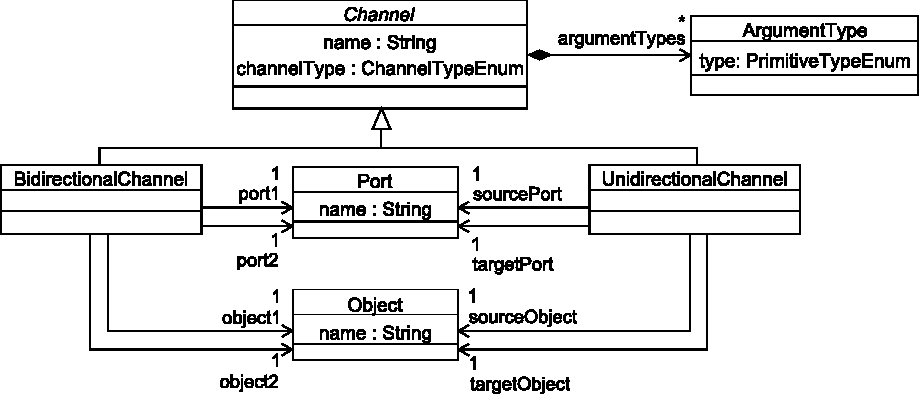
\includegraphics[scale=0.6]{slco/figs/metamodel/mm_slco_chan}
  \caption{Channels in \SLCO}
  \label{fig:slco:MMChan}
\end{figure}

Objects communicate with each other via channels, which are either bidirectional or unidirectional.
\SLCO offers three types of channels: synchronous channels, asynchronous, lossy channels, and asynchronous, lossless channels.
Each asynchronous channel is implicitly associated to one or two one-place buffers.
A unidirectional channel is associated to one buffer, and a bidirectional channel is associated to two buffers, one for each direction.
Signals can be sent over an asynchronous, lossless channel in a certain direction if the buffer associated to that direction is empty.
If a buffer is not empty, statements that send signals over this buffer block.
Signals can always be sent over asynchronous, lossy channels.
Because these channels are lossy, however, some signals sent over these channel are not stored in the corresponding buffer.
If the buffer corresponding to a channel already contains a signal and another signal is sent over this channel, the existing signal is replaced with the new signal.
If the buffer associated to a channel is empty, the signal reception statements that receive signals via this channel are blocked.
If the buffer associated to a channel contains a signal and a matching signal reception statement is executed, the signal is removed from the buffer and received by the state machine executing the signal reception statement.
A channel can only be used to send and receive signals with a certain signature, which defines the number of arguments of a signal and the types of these arguments.
The part of the \SLCO metamodel concerning channels is shown in Figure~\ref{fig:slco:MMChan}.

\begin{figure}[hbt]
 \centering
 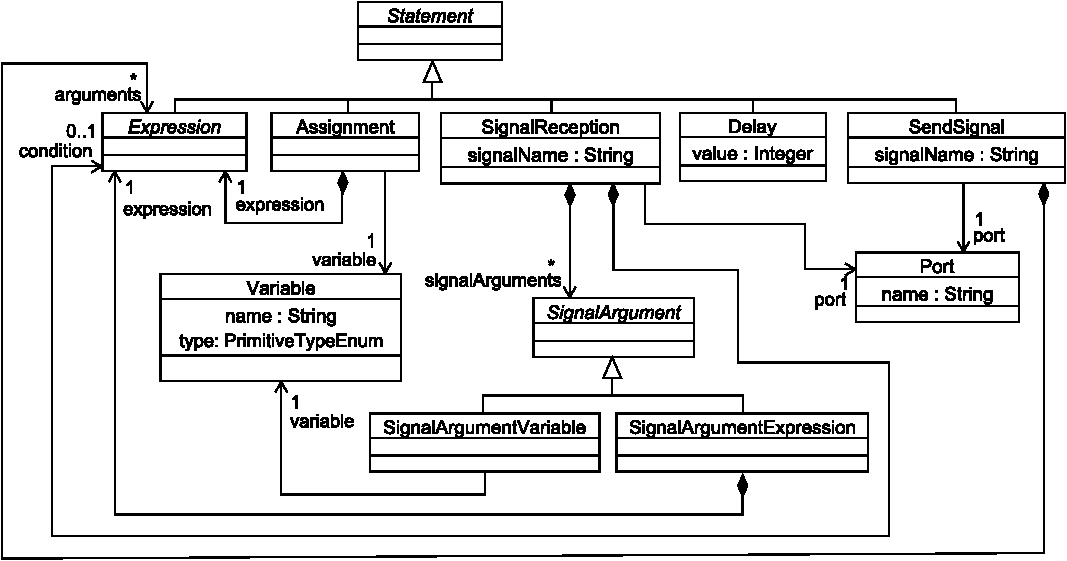
\includegraphics[scale=0.6]{slco/figs/metamodel/mm_slco_stat}
 \caption{Statements in \SLCO}
 \label{fig:slco:MMStatements}
\end{figure}

\SLCO offers five types of statements, as shown in Figure~\ref{fig:slco:MMStatements}.
A Boolean expression represents a statement that blocks the transition from a source to a target state until the expression evaluates to \SLCOTrue.
The part of the \SLCO metamodel concerning expressions is shown in Figure~\ref{fig:slco:MMExp}.
A delay statement blocks a transition until a specified amount of time measured in milliseconds has passed.
A transition with a (conditional) signal reception statement is enabled if a signal with appropriate arguments is received via the indicated port and the optional condition holds.
There are two ways of specifying that a signal reception is conditional.
First, expressions given as arguments of a signal reception specify that only signals whose argument values are equal to the corresponding expressions are accepted.
Second, only those signals are accepted for which the optional condition of a signal reception evaluates to \SLCOTrue.
This condition is a Boolean expression that may refer to the arguments of the signal that is offered via the port.
Besides these statements, \SLCO also offers statements for assigning values to variables and for sending signals via ports.

\begin{figure}[hbt]
  \centering
  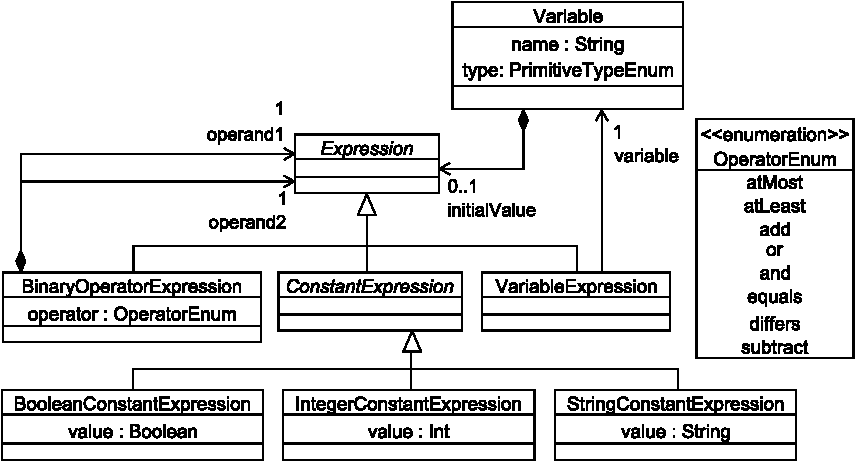
\includegraphics[scale=0.6]{slco/figs/metamodel/mm_slco_exp}
  \caption{Expressions in \SLCO}
  \label{fig:slco:MMExp}
\end{figure}

